% Graph: L2 distance distribution with regard to Model families
% Distance metric distributions across different model families
\begin{figure*}[!t]
    \centering
    % L2 Distance
    \begin{subfigure}{0.5\textwidth}
        \centering
        \begin{subfigure}{0.2\textwidth}
            \centering
            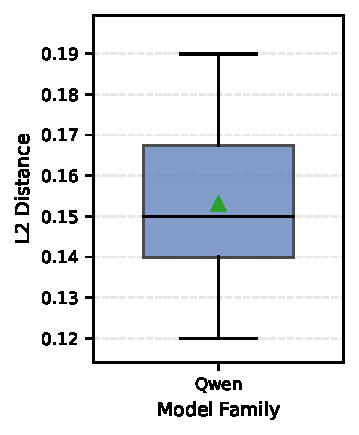
\includegraphics[width=\textwidth]{fig/rq1_qwen_l2_boxplot.pdf}
            \caption*{Qwen}
        \end{subfigure}%
        \hfill
        \begin{subfigure}{0.2\textwidth}
            \centering
            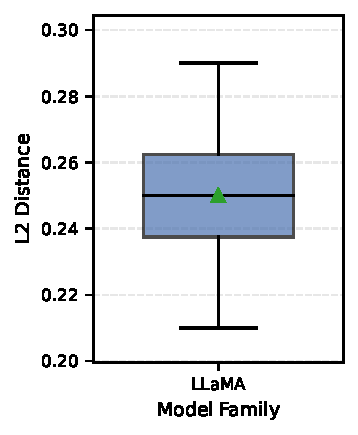
\includegraphics[width=\textwidth]{fig/rq1_llama_l2_boxplot.pdf}
            \caption*{LLaMA}
        \end{subfigure}%
        \hfill
        \begin{subfigure}{0.2\textwidth}
            \centering
            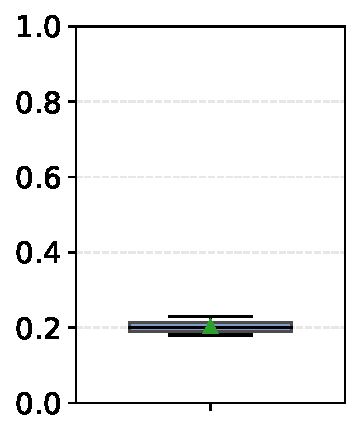
\includegraphics[width=\textwidth]{fig/rq1_granite_l2_boxplot.pdf}
            \caption*{Granite}
        \end{subfigure}%
        \hfill
        \begin{subfigure}{0.2\textwidth}
            \centering
            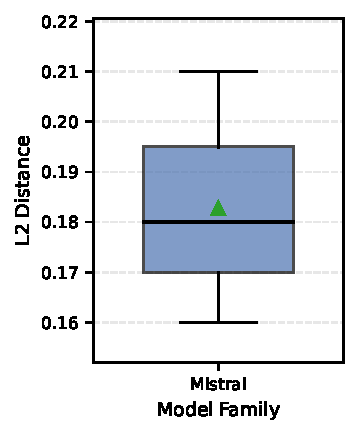
\includegraphics[width=\textwidth]{fig/rq1_mistral_l2_boxplot.pdf}
            \caption*{Mistral}
        \end{subfigure}%
        \hfill
        \begin{subfigure}{0.2\textwidth}
            \centering
            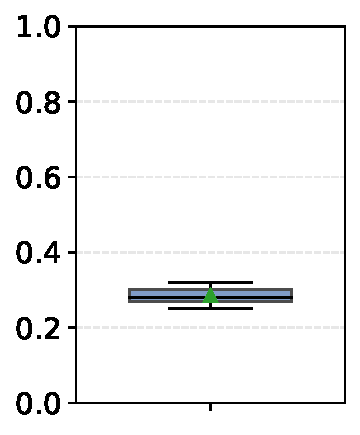
\includegraphics[width=\textwidth]{fig/rq1_others_l2_boxplot.pdf}
            \caption*{Others}
        \end{subfigure}
        \caption{L2 Distance}
        \label{fig:rq1-l2-boxplots}
    \end{subfigure}%
    % Cosine Similarity
    \begin{subfigure}{0.5\textwidth}
        \centering
        \begin{subfigure}{0.2\textwidth}
            \centering
            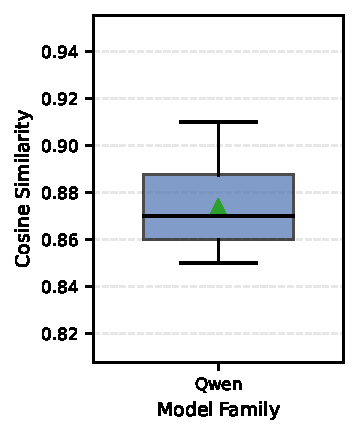
\includegraphics[width=\textwidth]{fig/rq1_qwen_cos_boxplot.pdf}
            \caption*{Qwen}
        \end{subfigure}%
        \hfill
        \begin{subfigure}{0.2\textwidth}
            \centering
            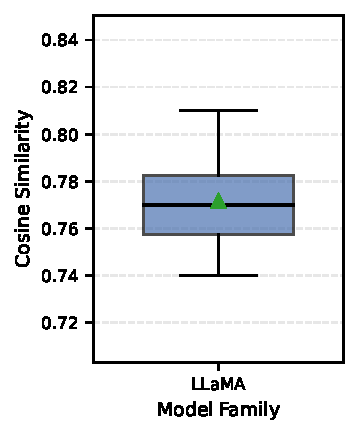
\includegraphics[width=\textwidth]{fig/rq1_llama_cos_boxplot.pdf}
            \caption*{LLaMA}
        \end{subfigure}%
        \hfill
        \begin{subfigure}{0.2\textwidth}
            \centering
            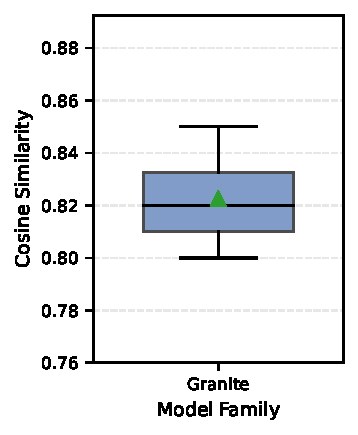
\includegraphics[width=\textwidth]{fig/rq1_granite_cos_boxplot.pdf}
            \caption*{Granite}
        \end{subfigure}%
        \hfill
        \begin{subfigure}{0.2\textwidth}
            \centering
            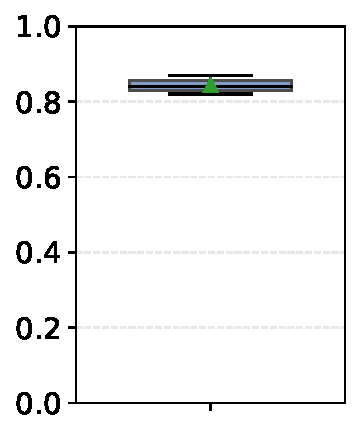
\includegraphics[width=\textwidth]{fig/rq1_mistral_cos_boxplot.pdf}
            \caption*{Mistral}
        \end{subfigure}%
        \hfill
        \begin{subfigure}{0.2\textwidth}
            \centering
            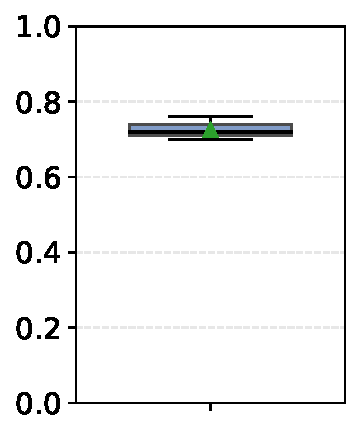
\includegraphics[width=\textwidth]{fig/rq1_others_cos_boxplot.pdf}
            \caption*{Others}
        \end{subfigure}%
        \caption{Cosine Similarity}
        \label{fig:rq1-cos-boxplots}
    \end{subfigure}
    % \vspace{0.3cm}
    % Abs Mean
    \begin{subfigure}{0.49\textwidth}
        \centering
        \begin{subfigure}{0.2\textwidth}
            \centering
            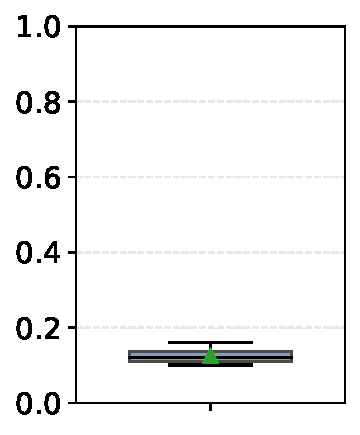
\includegraphics[width=\textwidth]{fig/rq1_qwen_abs_mean_boxplot.pdf}
            \caption*{Qwen}
        \end{subfigure}%
        \hfill
        \begin{subfigure}{0.2\textwidth}
            \centering
            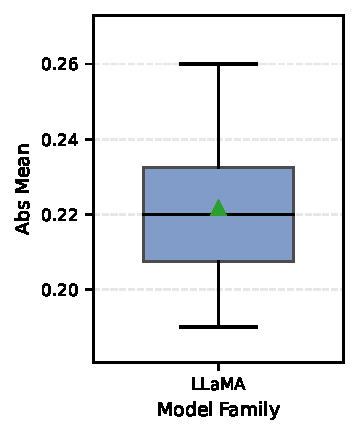
\includegraphics[width=\textwidth]{fig/rq1_llama_abs_mean_boxplot.pdf}
            \caption*{LLaMA}
        \end{subfigure}%
        \hfill
        \begin{subfigure}{0.2\textwidth}
            \centering
            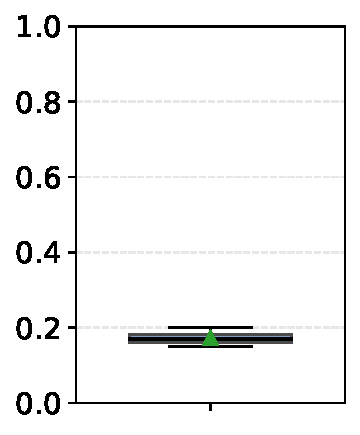
\includegraphics[width=\textwidth]{fig/rq1_granite_abs_mean_boxplot.pdf}
            \caption*{Granite}
        \end{subfigure}%
        \hfill
        \begin{subfigure}{0.2\textwidth}
            \centering
            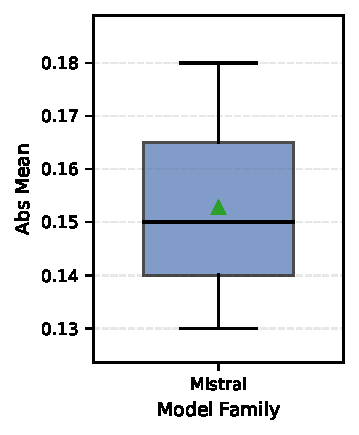
\includegraphics[width=\textwidth]{fig/rq1_mistral_abs_mean_boxplot.pdf}
            \caption*{Mistral}
        \end{subfigure}%
        \hfill
        \begin{subfigure}{0.2\textwidth}
            \centering
            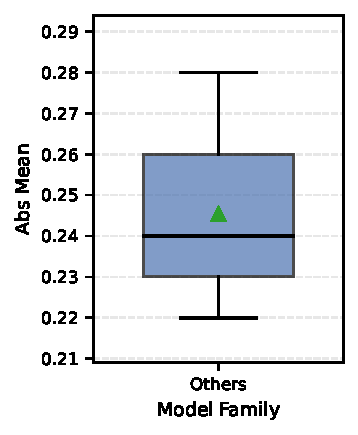
\includegraphics[width=\textwidth]{fig/rq1_others_abs_mean_boxplot.pdf}
            \caption*{Others}
        \end{subfigure}%
        \caption{Abs Mean}
        \label{fig:rq1-abs-mean-boxplots}
    \end{subfigure}
    % Abs Max
    \begin{subfigure}{0.49\textwidth}
        \centering
        \begin{subfigure}{0.2\textwidth}
            \centering
            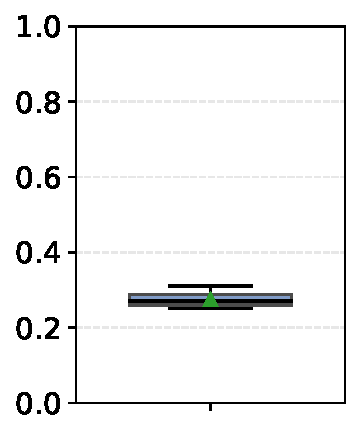
\includegraphics[width=\textwidth]{fig/rq1_qwen_abs_max_boxplot.pdf}
            \caption*{Qwen}
        \end{subfigure}%
        \hfill
        \begin{subfigure}{0.2\textwidth}
            \centering
            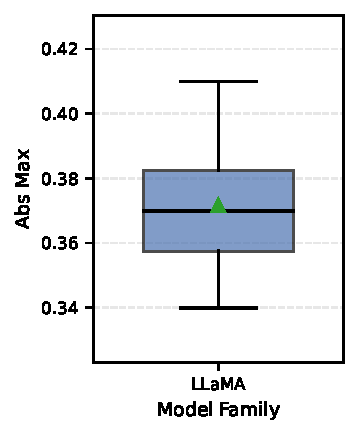
\includegraphics[width=\textwidth]{fig/rq1_llama_abs_max_boxplot.pdf}
            \caption*{LLaMA}
        \end{subfigure}%
        \hfill
        \begin{subfigure}{0.2\textwidth}
            \centering
            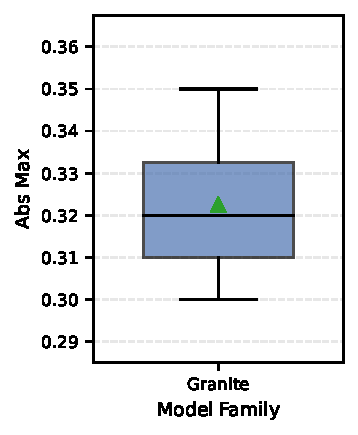
\includegraphics[width=\textwidth]{fig/rq1_granite_abs_max_boxplot.pdf}
            \caption*{Granite}
        \end{subfigure}%
        \hfill
        \begin{subfigure}{0.2\textwidth}
            \centering
            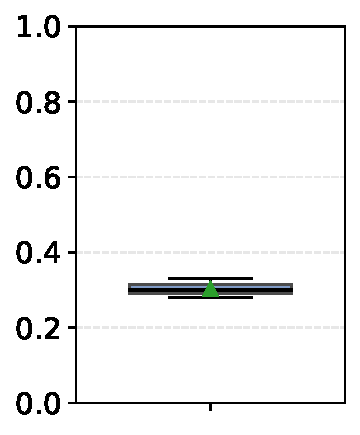
\includegraphics[width=\textwidth]{fig/rq1_mistral_abs_max_boxplot.pdf}
            \caption*{Mistral}
        \end{subfigure}%
        \hfill
        \begin{subfigure}{0.2\textwidth}
            \centering
            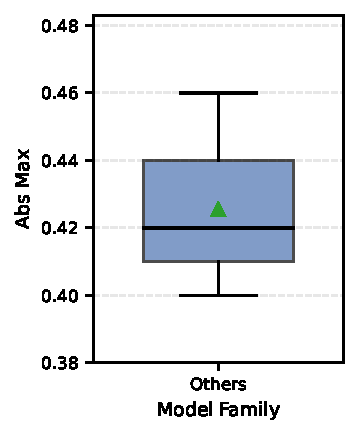
\includegraphics[width=\textwidth]{fig/rq1_others_abs_max_boxplot.pdf}
            \caption*{Others}%
        \end{subfigure}
        \caption{Abs Max}
        \label{fig:rq1-abs-max-boxplots}
    \end{subfigure}
    % \vspace{0.3cm}
    % Sparse Abs.
    \begin{subfigure}{0.49\textwidth}
        \centering
        \begin{subfigure}{0.2\textwidth}
            \centering
            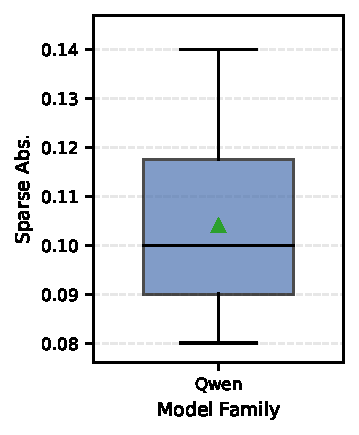
\includegraphics[width=\textwidth]{fig/rq1_qwen_sparse_abs_boxplot.pdf}
            \caption*{Qwen}
        \end{subfigure}%
        \hfill
        \begin{subfigure}{0.2\textwidth}
            \centering
            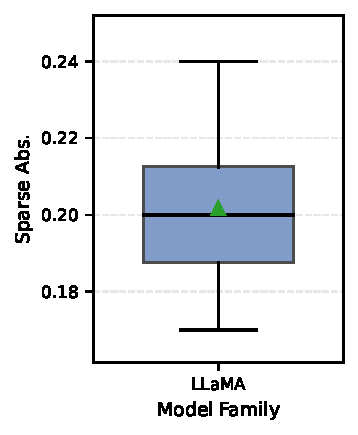
\includegraphics[width=\textwidth]{fig/rq1_llama_sparse_abs_boxplot.pdf}
            \caption*{LLaMA}
        \end{subfigure}%
        \hfill
        \begin{subfigure}{0.2\textwidth}
            \centering
            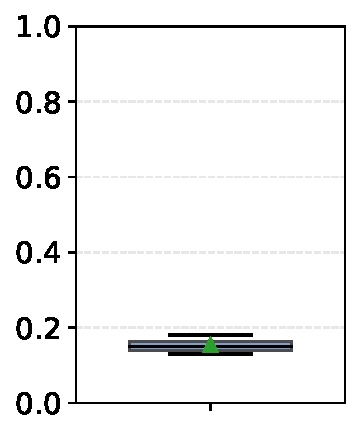
\includegraphics[width=\textwidth]{fig/rq1_granite_sparse_abs_boxplot.pdf}
            \caption*{Granite}
        \end{subfigure}%
        \hfill
        \begin{subfigure}{0.2\textwidth}
            \centering
            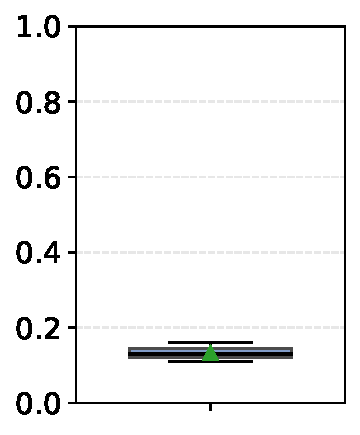
\includegraphics[width=\textwidth]{fig/rq1_mistral_sparse_abs_boxplot.pdf}
            \caption*{Mistral}
        \end{subfigure}%
        \hfill
        \begin{subfigure}{0.2\textwidth}
            \centering
            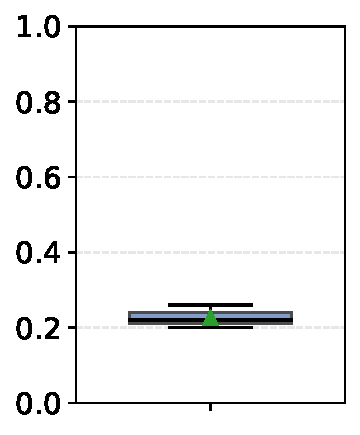
\includegraphics[width=\textwidth]{fig/rq1_others_sparse_abs_boxplot.pdf}
            \caption*{Others}
        \end{subfigure}
        \caption{Sparse Abs.}
        \label{fig:rq1-sparse-abs-boxplots}
    \end{subfigure}
    % \vspace{0.3cm}
    % Sparse Rel.
    \begin{subfigure}{0.49\textwidth}
        \centering
        \begin{subfigure}{0.2\textwidth}
            \centering
            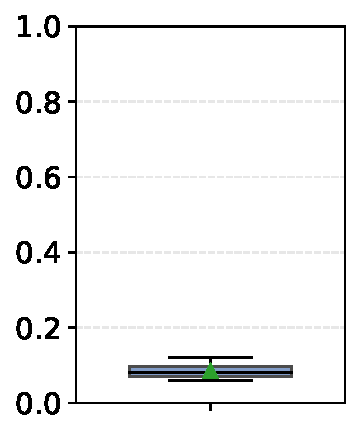
\includegraphics[width=\textwidth]{fig/rq1_qwen_sparse_rel_boxplot.pdf}
            \caption*{Qwen}
        \end{subfigure}%
        \hfill
        \begin{subfigure}{0.2\textwidth}
            \centering
            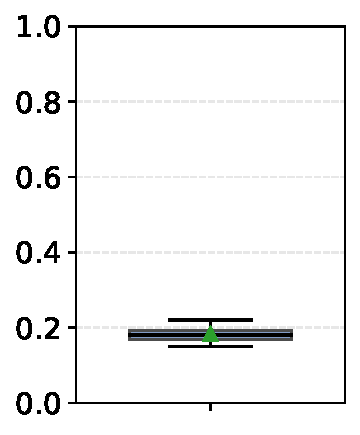
\includegraphics[width=\textwidth]{fig/rq1_llama_sparse_rel_boxplot.pdf}
            \caption*{LLaMA}
        \end{subfigure}%
        \hfill
        \begin{subfigure}{0.2\textwidth}
            \centering
            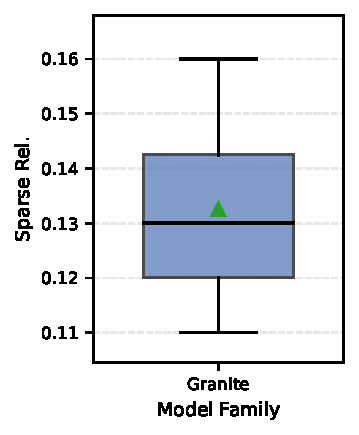
\includegraphics[width=\textwidth]{fig/rq1_granite_sparse_rel_boxplot.pdf}
            \caption*{Granite}
        \end{subfigure}%
        \hfill
        \begin{subfigure}{0.2\textwidth}
            \centering
            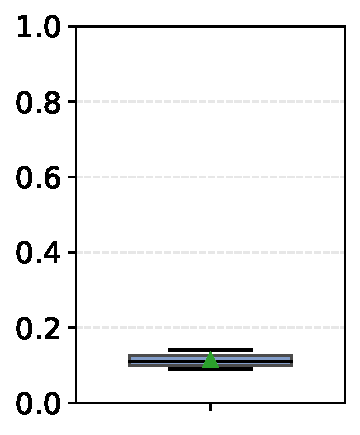
\includegraphics[width=\textwidth]{fig/rq1_mistral_sparse_rel_boxplot.pdf}
            \caption*{Mistral}
        \end{subfigure}%
        \hfill
        \begin{subfigure}{0.2\textwidth}
            \centering
            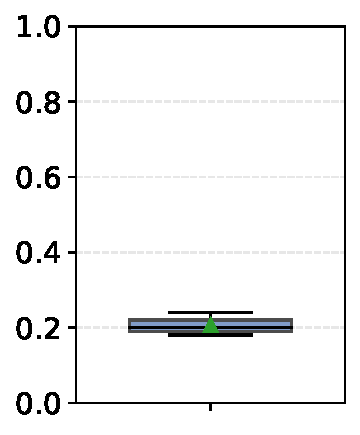
\includegraphics[width=\textwidth]{fig/rq1_others_sparse_rel_boxplot.pdf}
            \caption*{Others}
        \end{subfigure}
        \caption{Sparse Rel.}
        \label{fig:rq1-sparse-rel-boxplots}
    \end{subfigure}
    \caption{Distance metric distributions across different model families (RQ1).}
    \label{fig:rq1-all-metrics-boxplots}
\end{figure*}